\chapter{Modello delle Forze e Momenti Aerodinamici}
Le forze $\mathbf{F}$ e i momenti $\mathbf{M}$ presenti nelle equazioni dinamiche del Capitolo 3 sono la somma dei contributi aerodinamici (pedice $A$) e propulsivi (pedice $T$, \textit{Thrust}). Essendo la gravità già esplicitata nelle equazioni traslazionali, si ha:

\begin{align}
	\mathbf{F} &= \mathbf{F}_A + \mathbf{F}_T \\
	\mathbf{M} &= \mathbf{M}_A + \mathbf{M}_T
\end{align}
Questo capitolo definisce le componenti aerodinamiche secondo la convenzione standard di Stevens e Lewis


\section{Pressione Dinamica e Geometria di Riferimento}
\label{capitolo3}
Le forze aerodinamiche scalano con l'energia cinetica del flusso d'aria. Si definisce la pressione dinamica $\bar{q}$ attraverso la seguente relazione, la cui scomposizione vettoriale è illustrata concettualmente nella \hyperref[fig:liftforce]{Figura \ref*{fig:liftforce}}:

\begin{equation}
	\bar{q} = \frac{1}{2} \rho V_T^2
\end{equation}

dove $\rho$ è la densità dell'aria e $V_T$ la \textit{True Airspeed}. I parametri geometrici di riferimento del velivolo necessari per il calcolo dei coefficienti adimensionali sono:

\begin{itemize}
	\item $S$: Superficie alare di riferimento (\textit{Wing reference area}).
	\item $\bar{c}$: Corda aerodinamica media (\textit{Mean aerodynamic chord}), usata per adimensionalizzare il momento di beccheggio.
	\item $b$: {Apertura alare (\textit{Wingspan})}, usata per adimensionalizzare i momenti di rollio e imbardata (come visibile nella \hyperref[fig:wingspan]{Figura \ref*{fig:wingspan}}).
\end{itemize}


\begin{figure}[H]
	\centering
	
\includegraphics[width=0.7\linewidth]{foto/photo/liftForce}
	\caption{Rappresentazione delle forze aerodinamiche incidenti sul profilo alare e scomposizione del vettore velocità.}
	\label{fig:liftforce}
\end{figure}

\begin{figure}[H]
	\centering
	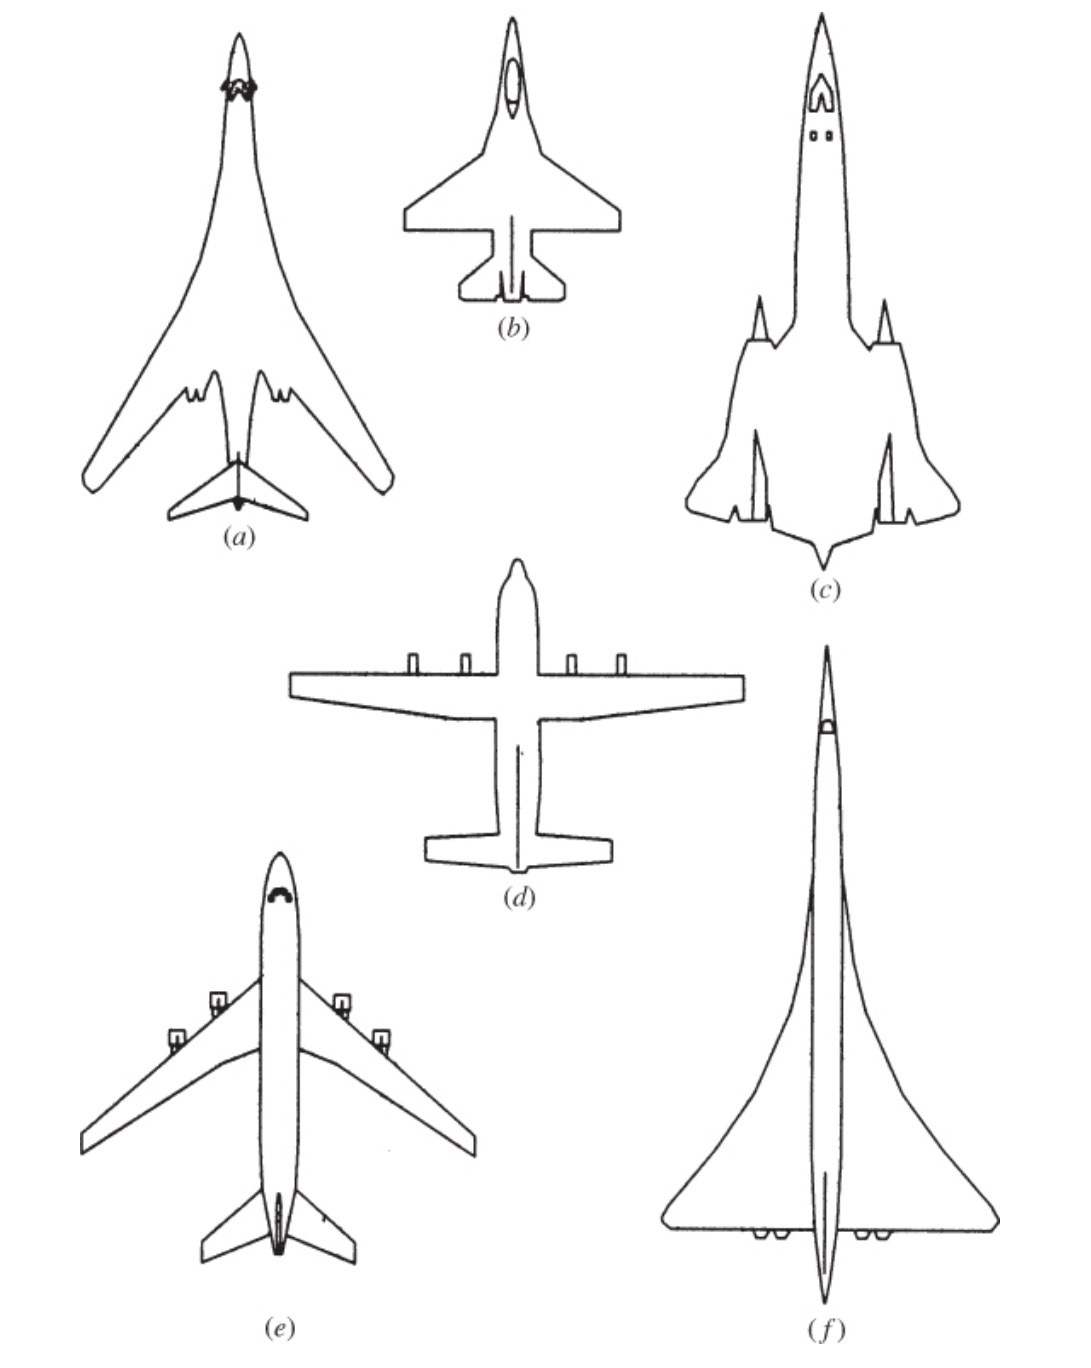
\includegraphics[width=0.45\linewidth]{Foto/photo/wing_span}
	\caption{Rappresentazione geometrica dell'apertura alare ($b$) e dei parametri di riferimento del velivolo.}
	\label{fig:wingspan}
\end{figure}



\section{Modelli di forze aerodinamiche}
Le forze aerodinamiche nel Body Frame sono espresse tramite i coefficienti adimensionali $C_X, C_Y, C_Z$:
\begin{align}
	F_{xA} &= \bar{q} S C_X \\
	F_{yA} &= \bar{q} S C_Y \\
	F_{zA} &= \bar{q} S C_Z
\end{align}

Tradizionalmente, in galleria del vento, i dati vengono estratti nel sistema di riferimento del vento (Wind Axes), dove le forze sono Portanza (\textit{Lift}, $L$), Resistenza (\textit{Drag}, $D$) e Forza Laterale (\textit{Side Force}, $Y$). Trascurando l'angolo di derapata ($\beta \approx 0$) per la dinamica longitudinale, la rotazione dal sistema Wind al sistema Body in funzione dell'angolo d'attacco $\alpha$ è:
\begin{align}
	C_X &= -C_D \cos\alpha + C_L \sin\alpha \\
	C_Z &= -C_D \sin\alpha - C_L \cos\alpha
\end{align}
\textbf{Nota bene:} Si presti attenzione al segno di $C_Z$. Essendo l'asse $Z_B$ puntato verso il basso (convenzione FRD), una portanza positiva (diretta verso l'alto) genera un $F_{zA}$ negativo.

\section{Adimensionalizzazione dei momenti}
I momenti aerodinamici attorno al baricentro dipendono dai coefficienti di rollio ($C_l$), beccheggio ($C_m$) e imbardata ($C_n$). Per adimensionalizzare i ratei di rotazione, si utilizzano i fattori $\frac{b}{2V_T}$ per la dinamica latero-direzionale e $\frac{\bar{c}}{2V_T}$ per la longitudinale:
\begin{align}
	L_A &= \bar{q} S b C_l \\
	M_A &= \bar{q} S \bar{c} C_m \\
	N_A &= \bar{q} S b C_n
\end{align}

\section{Analisi delle derivate di stabilità tramite serie di Taylor}
Per simulazioni o sintesi di controllori lineari, i coefficienti aerodinamici vengono espansi in serie di Taylor rispetto alle variabili di stato e di controllo

\subsection{Dinamica longitudinale}
\label{sec:coefficienti_aerodinamici}
I coefficienti longitudinali dipendono principalmente da $\alpha$, dal rateo di beccheggio $q$ e dal comando dell'equilibratore $\delta_e$:
\subsection{Modello Aerodinamico e Derivate di Stabilità}
\label{sec:derivate_aerodinamiche}

Nelle equazioni del moto precedentemente ricavate, le forze e i momenti aerodinamici sono racchiusi all'interno dei coefficienti globali. Per esplicitare la dipendenza di tali carichi dallo stato del velivolo e dall'ingresso di controllo, è necessario espandere i coefficienti tramite un approccio alle piccole perturbazioni (Serie di Taylor arrestata al primo ordine). Come documentato nel modello NASA dell'F-16 (Stevens e Lewis), i dati aerodinamici del velivolo sono tipicamente strutturati fornendo i coefficienti delle forze direttamente proiettati in \textit{Assi Corpo} ($C_X, C_Z$), piuttosto che in assi vento ($C_D, C_L$). L'espansione lineare dei coefficienti longitudinali risulta pertanto:

\begin{align}
	C_X &= C_{X_0}(\alpha) + C_{X_q} \left(\frac{q \bar{c}}{2 V_T}\right) + C_{X_{\delta e}} \delta_e \label{eq:Cx_exp} \\
	C_Z &= C_{Z_0}(\alpha) + C_{Z_q} \left(\frac{q \bar{c}}{2 V_T}\right) + C_{Z_{\delta e}} \delta_e \label{eq:Cz_exp} \\
	C_m &= C_{m_0} + C_{m_\alpha} \alpha + C_{m_q} \left(\frac{q \bar{c}}{2 V_T}\right) + C_{m_{\delta e}} \delta_e \label{eq:Cm_exp}
\end{align}

Questa formulazione scompone matematicamente l'aerodinamica in tre contributi fisici distinti, fondamentali per la successiva costruzione delle matrici di stato $\mathbf{A}_{long}$ e di ingresso $\mathbf{B}_{long}$:

\begin{itemize}
	\item \textbf{Aerodinamica Statica Base ($C_{X_0}, C_{Z_0}, C_{m_0} + C_{m_\alpha}\alpha$):} Rappresentano i carichi generati dal velivolo in volo stazionario. Il termine $C_{m_\alpha}$ è la derivata di stabilità statica longitudinale: per un velivolo convenzionale stabile deve essere negativo (un aumento di incidenza genera un momento picchiante di richiamo), ma nel caso dell'F-16, intrinsecamente instabile nel volo subsonico, tale termine risulta positivo, rendendo obbligatoria la presenza di un sistema SAS (Stability Augmentation System).
	
	\item \textbf{Derivate di Smorzamento Dinamico ($C_{X_q}, C_{Z_q}, C_{m_q}$):} Moltiplicate per il rateo di beccheggio adimensionalizzato ($q \bar{c}/2 V_T$), modellano gli effetti instazionari dovuti alla rotazione del velivolo. Il termine dominante è $C_{m_q}$ (\textit{Pitch Damping}), che quantifica l'opposizione aerodinamica del piano di coda al moto di beccheggio, agendo come uno smorzatore viscoso naturale.
	
	\item \textbf{Derivate di Controllo ($C_{X_{\delta e}}, C_{Z_{\delta e}}, C_{m_{\delta e}}$):} Isolano l'effetto puro dell'elevatore. Il termine $C_{m_{\delta e}}$ costituisce l'efficacia di comando primaria per governare l'accelerazione angolare $\dot{q}$, mentre $C_{Z_{\delta e}}$ modella la variazione istantanea di forza normale sull'asse Z (responsabile del salto nell'accelerazione $a_z$ e della dinamica a non-minimo fase discussa in precedenza).
\end{itemize}

\textit{Nota di trasformazione:} Qualora le equazioni di stato impieghino le forze in assi vento (come nel caso delle derivate $\dot{V}_T$ e $\dot{\alpha}$), i coefficienti del modello tabellare in assi corpo vengono ruotati tramite le usuali trasformazioni trigonometriche:
\begin{align*}
	C_D &= -C_X \cos\alpha + C_Z \sin\alpha \\
	C_L &= -C_Z \cos\alpha - C_X \sin\alpha
\end{align*}

Il termine $C_{m_\alpha}$ rappresenta la rigidezza in beccheggio e definisce la stabilità statica longitudinale del velivolo, mentre $C_{m_q}$ (damping di beccheggio) fornisce la stabilità dinamica. Queste trasformazioni verranno utilizzate all'interno del capitolo 6 per ottenere le equazioni puntate del controllo longitudinale in assi del corpo, si spiega meglio in questo paragrafo \ref{sec:coeff_aero}.

\subsection{Dinamica Latero-Direzionale e Accoppiamento Aerodinamico}
\label{sec:derivate_latero_direzionali}

A differenza del moto longitudinale, che gode di un disaccoppiamento naturale dalle variabili laterali in condizioni di volo simmetrico, la dinamica latero-direzionale è intrinsecamente accoppiata. Un moto di rollio induce effetti sull'asse di imbardata e viceversa. Per modellare matematicamente le forze laterali ($Y$) e i momenti di rollio ($L$) e imbardata ($N$), i coefficienti adimensionali globali $C_Y, C_l, C_n$ vengono espansi in Serie di Taylor rispetto all'angolo di derapata (o slittamento) $\beta$, ai ratei angolari $p, r$ e agli ingressi di controllo asimmetrici (alettoni $\delta_a$ e timone $\delta_r$).

È fondamentale notare che, per i coefficienti latero-direzionali dipendenti dai ratei angolari, il parametro geometrico di adimensionalizzazione non è più la corda media aerodinamica $\bar{c}$ (utilizzata nel piano longitudinale), bensì l'apertura alare $b$. Le equazioni linearizzate assumono la seguente forma:

\begin{align}
	C_Y &= C_{Y_\beta} \beta + C_{Y_p} \left(\frac{p b}{2 V_T}\right) + C_{Y_r} \left(\frac{r b}{2 V_T}\right) + C_{Y_{\delta a}} \delta_a + C_{Y_{\delta r}} \delta_r \label{eq:Cy_exp} \\
	C_l &= C_{l_\beta} \beta + C_{l_p} \left(\frac{p b}{2 V_T}\right) + C_{l_r} \left(\frac{r b}{2 V_T}\right) + C_{l_{\delta a}} \delta_a + C_{l_{\delta r}} \delta_r \label{eq:Cl_exp} \\
	C_n &= C_{n_\beta} \beta + C_{n_p} \left(\frac{p b}{2 V_T}\right) + C_{n_r} \left(\frac{r b}{2 V_T}\right) + C_{n_{\delta a}} \delta_a + C_{n_{\delta r}} \delta_r \label{eq:Cn_exp}
\end{align}

Questo sistema evidenzia la natura intrinsecamente \textit{Multi-Input Multi-Output} (MIMO) dell'aerodinamica latero-direzionale. I contributi possono essere fisicamente scomposti in tre categorie principali:

\begin{itemize}
	\item \textbf{Derivate Statiche di Derapata ($\beta$):} Rappresentano la reazione del velivolo a un vento laterale. 
	\begin{itemize}
		\item $C_{n_\beta}$ (\textit{Stabilità Direzionale o Effetto Banderuola}): Garantita dalla deriva verticale, deve essere rigidamente positivo per un volo stabile. Un $\beta > 0$ (vento da destra) deve generare un momento imbardante positivo ($n > 0$) per riportare il muso nel vento.
		\item $C_{l_\beta}$ (\textit{Effetto Diedro}): Modella l'accoppiamento rollio-derapata. In aerei stabili è tipicamente negativo: uno scivolamento a destra ($\beta > 0$) genera una maggiore portanza sulla semiala destra, creando un momento di rollio a sinistra ($l < 0$) che tende a raddrizzare il velivolo. L'equilibrio tra $C_{l_\beta}$ e $C_{n_\beta}$ determina le caratteristiche dei modi dinamici di \textit{Dutch Roll} e spirale divergente.
	\end{itemize}
	
	\item \textbf{Derivate di Smorzamento e Accoppiamento ($p, r$):} Modellano l'aerodinamica instazionaria durante le rotazioni. 
	\begin{itemize}
		\item \textit{Smorzamenti diretti ($C_{l_p}, C_{n_r}$):} Sono lo smorzamento di rollio (dovuto all'imponente resistenza delle semiali a ruotare) e lo smorzamento di imbardata. Sono termini fortemente stabilizzanti (negativi).
		\item \textit{Accoppiamenti incrociati ($C_{l_r}, C_{n_p}$):} Modellano l'interazione tra gli assi. Ad esempio, $C_{l_r}$ (rollio indotto dall'imbardata) descrive come un'imbardata verso destra aumenti la velocità relativa della semiala sinistra, generando più portanza asimmetrica e causando un momento di rollio indotto.
	\end{itemize}
	
	\item \textbf{Derivate di Controllo ($\delta_a, \delta_r$):}
	\begin{itemize}
		\item $C_{l_{\delta a}}$ e $C_{n_{\delta r}}$ rappresentano rispettivamente l'autorità primaria degli alettoni sul rollio e del timone sull'imbardata.
		\item $C_{n_{\delta a}}$ modella il fenomeno dell'\textit{Imbardata Inversa} (Adverse Yaw): una deflessione degli alettoni per rollare genera un differenziale di resistenza indotta (l'alettone abbassato crea più resistenza) che trascina il muso dell'aereo nella direzione opposta alla virata voluta. Questo termine parassita impone la progettazione di un interconnettore alettoni-timone (ARI - Aileron Rudder Interconnect) nelle leggi di controllo fly-by-wire.
	\end{itemize}
\end{itemize}


